%describe how you evaluated to show that your approach was successful. You may need a methods section, a results section and a conclusion

This chapter reflects on the theoretical architecture created in the previous chapter. I will break down each component of the gateway and test individual functionality using available open source tools. Secondly I will compare my model against a study 3GPP\footnote{http://www.3gpp.org/} did on giving \gls{wrtc} clients access to \gls{ims}, which is similar to this case. Then I will discuss the results and derive some guidelines.

\section{Evaluating the proposed gateway}
In this section a lot of experiments were conducted using sipml5\footnote{http://sipml5.org/}, which is an open-source HTML5 SIP client using \gls{rtcweb} for the media stack. It uses a SIP proxy for translating the signaling, a RTCWebBreaker to convert the media streams, and a media coder for transcoding. It operates very similar to my proposed architecture. In addition to that it connects to any SIP endpoint directly from the browser.

\subsection{The Signaling proxy}
In the signaling component a proxy solution was proposed to use a SIP stack for Javascript running over WebSockets. Using sipml5 and a range of different desktop SIP clients I tested to see how well the SIP proxy worked.   

\begin{table}[h]
\resizebox{\textwidth}{!}{%
\begin{tabular}{|p{1.3cm}|l|l|p{4cm}|p{4cm}|p{5cm}|}
\hline
SIP desktop clients & Audio & Video  & Latency                                                                                         & Quality                                                  & Comments                                                                                                            \\ \hline
Ekiga               & g.711 & failed & none                                                                                            & good audio quality                                       & did not get video working                                                                                           \\ \hline
Zoiper              & g.711 & vp8    & none for audio, video took approximately 5 seconds to appear, but then it was a live connection & good audio quality, huge packet loss on the video stream & crashed after just a few seconds during video conference                                                            \\ \hline
Jitsi               & g.711 & failed & none                                                                                            & good audio quality                                       & connection failed every time the application tried to negotiate a video codec, but worked fine when disabling video \\ \hline
Blink               & opus  & failed & none                                                                                            & good audio quality                                       & did not get video working                                                                                           \\ \hline
\end{tabular}
}
\caption{SIP desktop client interaction with web client using proxy and RTCWEB}
\label{tbl:sip-client-webrtc-interaction}
\end{table}

In figure \ref{tbl:sip-client-webrtc-interaction} the audio and video columns refer to the mutually agreed upon codec to be used during the signaling process. Since g.711 is the most preferred codec to be used in \gls{voip} systems it is natural that audio most often defaults to this codec. Experiments with video conferencing was not very successful, it was difficult getting a normal video session to work for various reasons, one of them being a mismatch in the \gls{sdp} which was noted in the interoperation chapter as a probable outcome. The one desktop client that did manage to get a working video session using the vp8 codec had a very high packet loss as seen in figure \ref{fig:wireshark-sip-call}. Reasons for this is hard to say as the experiment was done on a really good connection.

\begin{figure}[here]
\centerline{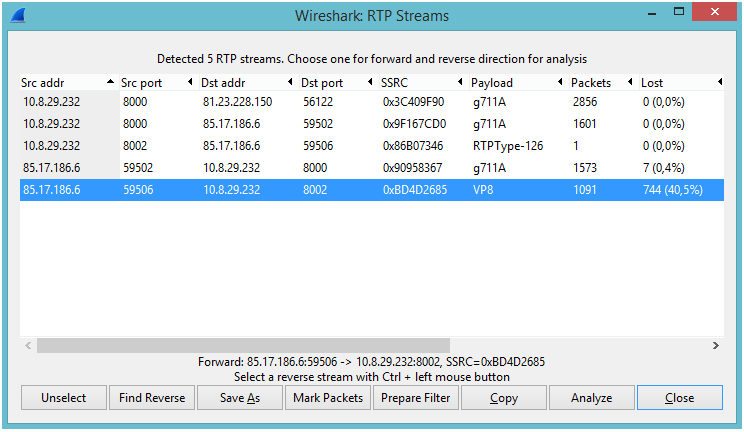
\includegraphics[scale=0.5]{wireshark-rtp.png}}
\caption{Wireshark analysis of a SIP call}
\label{fig:wireshark-sip-call}
\end{figure}

\subsection{The Transport Proxy}
Not much problems here, the connections were smooth with low latency even running behind a proxy. As mentioned earlier there was no problems doing audio calls, but video calling seemed to cause some problems, but these are probably not related to this component.

%%FYLL UT %%

\subsection{The Media Transcoder}
Since transcoding can be done in the cloud, the quality should not really be affected by this component. It is limited by which codec and your geographic location.

%%FYLL UT%%

\section{Evaluate against criteria defined by 3GPP}
What is IMS?

Why IMS? Almost all telco companies are exploring ways to provide webrtc-based access to legacy infrastructure/services they already have in palce.
These existing real-time communciation systems is or will be IMS based in most cases.

The 3gpp has started the technical definition of a solutuion for a webrtc client to access ims networks through the internet

This diagram depicts the reference architecture adopted:
3gpp tr 23.701 \ref output to date. work in progress

\begin{figure}[here]
\centerline{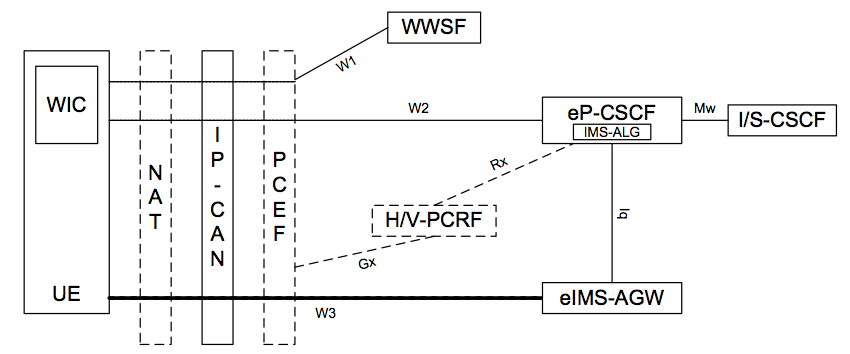
\includegraphics[scale=0.5]{3gpp-wrtc-ims-architecture.png}}
\caption{WebRTC IMS architecture}
\label{fig:wrtc-ims-architecture}
\end{figure}

Let's look at the main elements:

\textbf{WebRTC IMS Client (WIC)}
is downloaded from the wwsf. provides the aplpication logic and webrtc api calls to access communication services of ims. work on any device supproting a browser that supports webrtc.

\textbf{User Equipment(UE)}
UE device or applicationn can be a web application running on a browser.

\textbf{WebRTC Web Server Function (WWSF)}
from where the web client is downloaded.
or web server hosting the wic

\textbf{P-CSCF enhanced for WebRTC (eP-CSCF)}
entry point of SIP requests. add capacity to receive SIP over WebSockets
works as the signaling gateway. adapts signaling ont he webrtc side to standard ims-sip

\textbf{IMS Access Gateway enhanced for WebRTC (eIMS-AGW)}
supports webrtc media as defined by ietf
essentially the media gateway function.
supprot
dtls.-srtp    sdes is used in ims w keys in the signaling plane
auido/video transcoding  h.264 is supproted by h.264
rtcp multiplexing webrtc supports multiplexing of audio/video calls and rtp/rtcp over same rtp session and port. not supported in ims. must support demultiplexing

must also support negotiating ice candidates including stun and turn

the specification is open to the use of different protocols.

\textbf{IP Connectivity Access Network (IP-CAN)}
IP network used to reach the IMS core from the UE. Can be LTE for mobile, DSL and WLAN

\textbf{Policy and Charging Rules Function (PCRF) and Policy and Charging Enforcement Function (PCEF)}
supports policy and charging control decisions based on session and media-related information obtained from the P-CSCF.
Used deep packet inspection and decides based on rules whether the traffic is allowed or not.

\textbf{Network Address Translation (NAT)}
The WIC would noramlly be behind a NAT element so a box has been included in the diagram. ICE is used to enable two-way flows of srtp nehind nat so media gateway is used to exchange media flows with the ims core must support it.


\section{Results}
%Derived guidelines
this section presents guidelines and general recommendations on implementing the gateway


sip does not winterwork very well
almost all cases the sdp was the point of failure
or therer could be an agremement on an appropriate codec

\section{Conclusion}
%Peke på veien videre for å få verifisert dine anbefalinger - lead into future chapt